% Chapter Template

\chapter{Validation and Transferability Properties of DeepBM: A Study on Syndiotactic Polystyrene} % Main chapter title

\label{bm_ps} % Change X to a consecutive number; for referencing this chapter elsewhere, use \ref{ChapterX}

\section{Backmapping of Equilibrated Molecular Structures}


\subsection{Set-up and Reference Data}

\begin{figure}
  \centering
  \captionsetup{width=1.0\linewidth}
      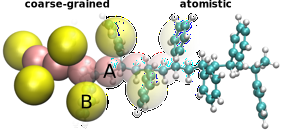
\includegraphics[width=0.70\textwidth]{./Figures/adversarial_backmapping/intro.pdf}
  \caption{\cite{stieffenhofer2020adversarial}}
  \label{fig_bm_intro}
\end{figure}

\subsection{Results}

\begin{figure}
  \centering
  \captionsetup{width=1.0\linewidth}
      \includegraphics[width=1.05\textwidth]{./Figures/adversarial_backmapping/sPS_temp_trans/ff_dists_and_rdf.pdf}
  \caption{ Canonical distributions for various force-field interaction terms at (left) $T$ = 568 K, (middle) $T$ = 453 K and (right) $T$ = 313 K for reference structures (black), structures generated with the baseline, energy-minimization-based backmapping method (red), and the new method DBM (blue). The model is trained solely on the high temperature data (left), but deployed at lower temperatures (middle and right). (a)–(c) C-C-C backbone angle, (d)–(f) C-C-C-C backbone dihedral, (g)–(i) C-C-C-C improper dihedral, (j)–(l) Lennard-Jones energies, and (m)–(o) radial distribution functions, g(r), of the non-bonded carbon atoms.\cite{stieffenhofer2020adversarial}}
  \label{fig_bm_intro}
\end{figure}

\subsection{Discussion}

\section{Temperature Transferability: From Melt to Crystal}

\begin{figure}
  \centering
      \includegraphics[width=0.6\textwidth]{./Figures/adversarial_backmapping/sPS_temp_trans/ps_polymorphs.pdf}
  \caption{Polymorphism of Polystyrene. At high temperature ($T$ = 568 K) the system stabilizes an amorphous phase. At lower temperatures the CG model mostly stabilizes the $\alpha$ polymorph at $T$ = 453 K and the $\beta$ polymorph at $T$ = 313 K. DeepBackmap is trained solely on the high-temperature ensemble ($T$ = 568 K) and test its transferability to the lower temperatures. \cite{stieffenhofer2020adversarial}}
  \label{fig_bm_intro}
\end{figure}


\begin{figure}
  \centering
      \includegraphics[width=1.1\textwidth]{./Figures/adversarial_backmapping/sPS_temp_trans/sm_snapshots.pdf}
  \caption{ Low-dimensional structural space of condensed-phase configurations at (a) $T$ = 568 K, (b) $T$ = 453K and (c) $T$ = 313 K. For each panel, snapshots are backmapped from identical coarse-grained configurations, highlighting the overlap between reference and DeepBackmap, but disconnect from the baseline method.\cite{stieffenhofer2020adversarial}}
  \label{fig_bm_intro}
\end{figure}


\subsection{Set-up and Reference Data}

\subsection{Results}

\subsection{Discussion}

\section{Chemical Transferability: From Small Molecules to Polymers}

\subsection{Set-up and Reference Data}

\subsection{Results}

\begin{figure}
  \centering
  \captionsetup{width=1.0\linewidth}
      \includegraphics[width=1.05\textwidth]{./Figures/adversarial_backmapping/sPS_chem_trans/angles.pdf}
  \caption{ \cite{stieffenhofer2020adversarial}}
  \label{fig_bm_intro}
\end{figure}

\subsection{Discussion}
